% This is TBP on Ag(100):


%%%%%%%%%%%%%%%%%%%%%%%% old motiv overview %%%%%%%%%%%%%%%%%%%%%%%% 
% To achieve an optical identification of different molecular configurations, some possible arrangements have been modeled for Mono-, Di- and Tetramers.
% \begin{figure}[h]
%  \begin{center}
%   \includegraphics[width=\textwidth]{./images/nitro-porphin-pattern-models-phenyl-pattern}
%  \end{center}
% \caption{Some possible arrangement of di- and tetramers. The white bars and dots indicate the pattern one would observe highlighted in STM when the phenyl rings dominate the signal}
% \end{figure}
% 
% \begin{figure}[h]
%  \begin{center}
%   \includegraphics[width=\textwidth]{./images/nitro-porphin-pattern-models-buthyl-pattern}
%  \end{center}
% \caption{Some possible arrangement of di- and tetramers. Dots indicate the pattern one would observe highlighted in STM when the phenyl (white) and tert-buthyl groups (yellow) dominate the signal.}
% \end{figure}
% Comparing the models with the STM images shows a good agreement between model and image when the butylphenyl groups are dominant in the signal.
%%%%%%%%%%%%%%%%%%%%%%%% %%%%%%%%%%%%%%%%%%%%%%%%  %%%%%%%%%%%%%%%%%%


%%%%%%%%%%%%%%%%%%%%%%%%%%%%%%%%%%%%%%%%%%%%%%%%%%%%%%%%%
The models match the shape of the dimer very well and is accurate even the the quatermer case, where two dimers are attached parallel via their butylphenyl groups. The interaction between the butylphenyl groups is considered to be van der Waals like \cite{iacovita_controlling_2012}.

Model and image differ for the cross-shaped tetramers, where the model suggests a dark center and the image shows a non vanishing DOS within the bias voltage around the fermi level.

Some spectroscopy could be achieved that shows different typical features for different areas in the molecule. Note that the spectra were done for molecules sitting on a Ag(100) surface.
There is a clear indication, that the macrocylce of the molecule contributes to the broad peak in the dI/dV data at around \SI{1}{\V}, while the nitro groups dominate the spectra at around \SI{600}{\milli \V}. 
Look at the corresponding .pptx file for the spectra and the corresponding IGOR-files dimer/quatermer1-2 for the spectra.

Gently heating to  .... ???
%%%%%%%%%%%%%%%%%%%%%%%%%%%%%%%%%%%%%%%%%%%%%%%%%%%%%%%%%
When the copper is exchanged with silver to act as substrate, TBP behaves quite different. Although the distribution on the surface is homogeneous on the surface, the interaction between molecules look different. While on copper the most abundant binding motiv is the head-to-head dimer, this motiv does not appear on silver as often as on copper. Two other motivs emerge on silver.

One of them is the double-dimer.  While on copper, two molecules may form a dimer in head-to-head configuration, on silver some form tetramers that almost look like two parallely merged dimers. While one dimer looks like two ``U'''s with facing open ends ($\in \ni$), the other dimer is shifted to closely match the first dimer best and lies parallel.

%-------------- Add graphic to explain!-------------- 

One motiv looks like a cross - build out of four molecules, each of them rotated by \SI{90}{\degree} with respect to its preliminary neighbour. Although there is no atom directly in the center, the cross looks bright in its center (in STM), which is somehow counterintuitive. This motiv still remains unclear.

\begin{figure}[h]
 \begin{center}
  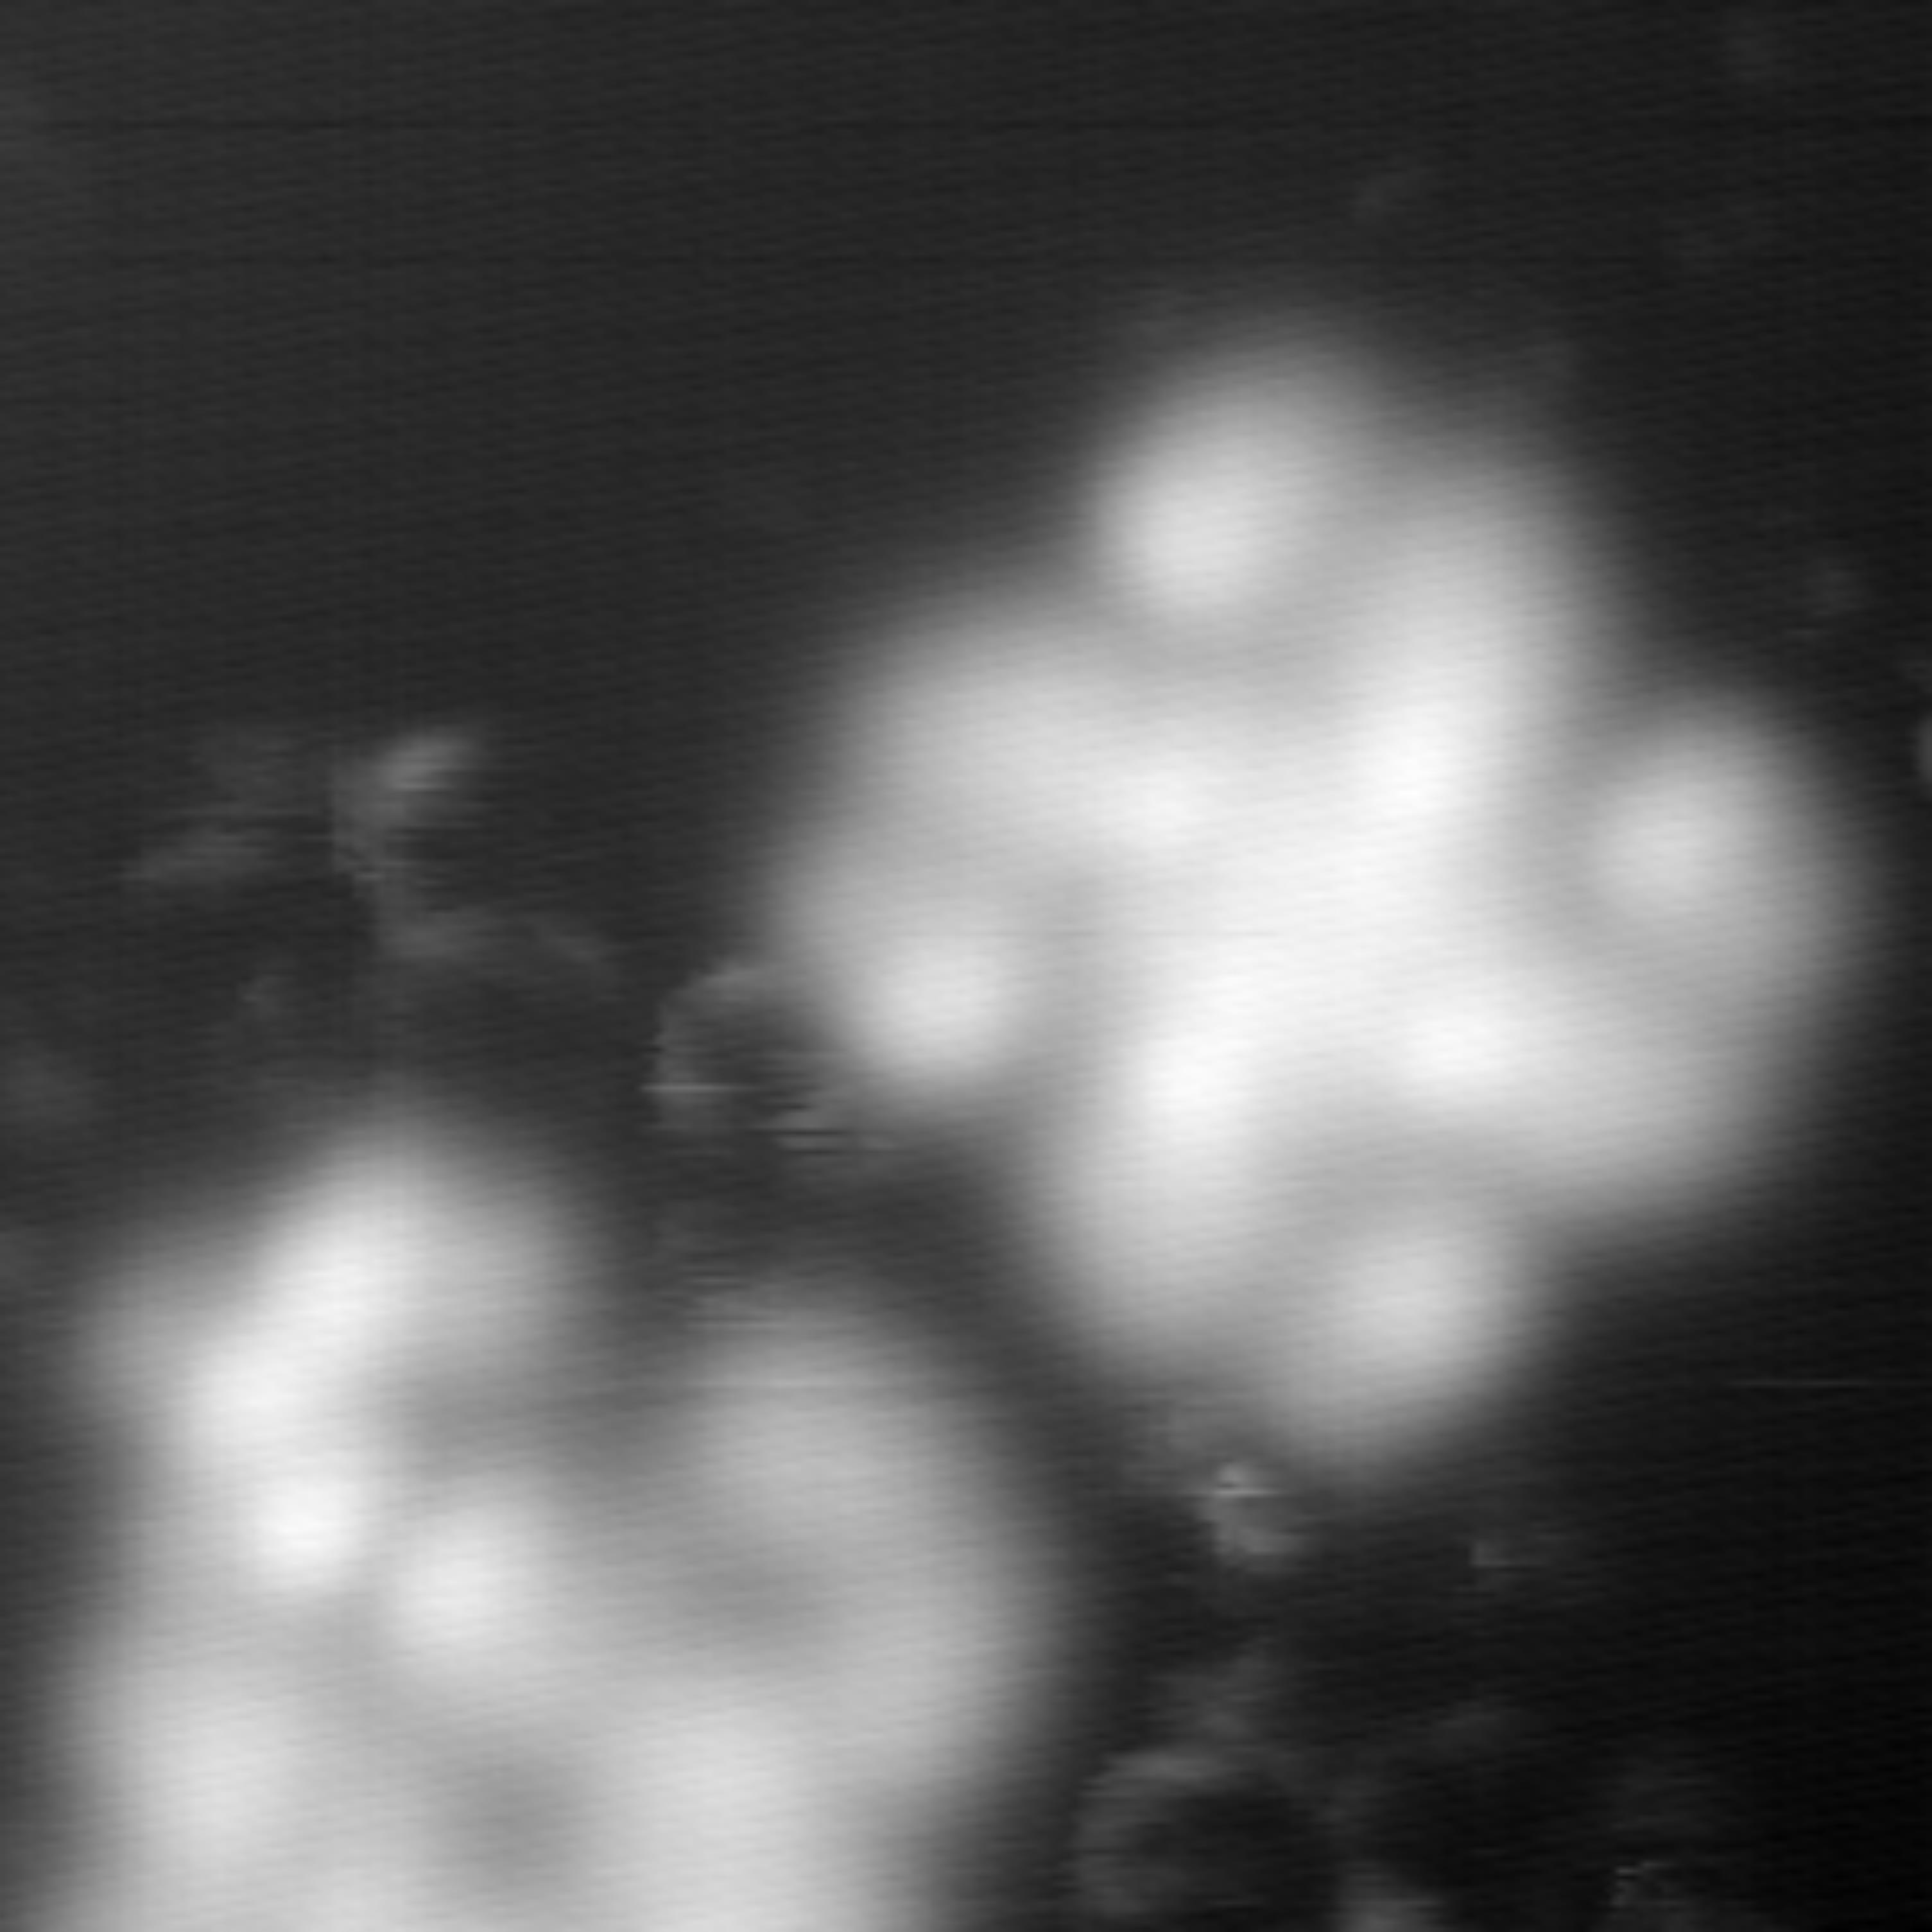
\includegraphics[width=0.5\textwidth]{./images/F150612-154558.jpg}
 \end{center}
\caption{\SI{13}\times\SI{13}{\nm \squared} image showing the formation of a TBP-dimer (lower left part of the image - ``head-to-head``) and a cross consisting of most likely 4 TBP molecules (upper right).}
\end{figure}

\begin{itemize}
 \item Butyl groups within TBP feature different contrasts (look rotated), while the orientation of the butyl-groups doesn't follow the close packed substrate rows. ---------------- find image and explain
 \item TBP molecules have been heated on silver substrate for \SI{10}{\minute} at \SI{170}{\degree \celsius}. The resulting sample did not feature chain-formation or improved ordering.
\end{itemize}

Only once an ordered area of TBP on Ag(100) was found, but its structure could not be resolved properly due to tip issues (compare figure \ref{fig:hex-TBP-Ag100}). Its unit cell looks hexagonal with roughly \SI{1.7} {\nano \meter} period in both unit cell directions. 

\begin{figure}[h]
 \centering
 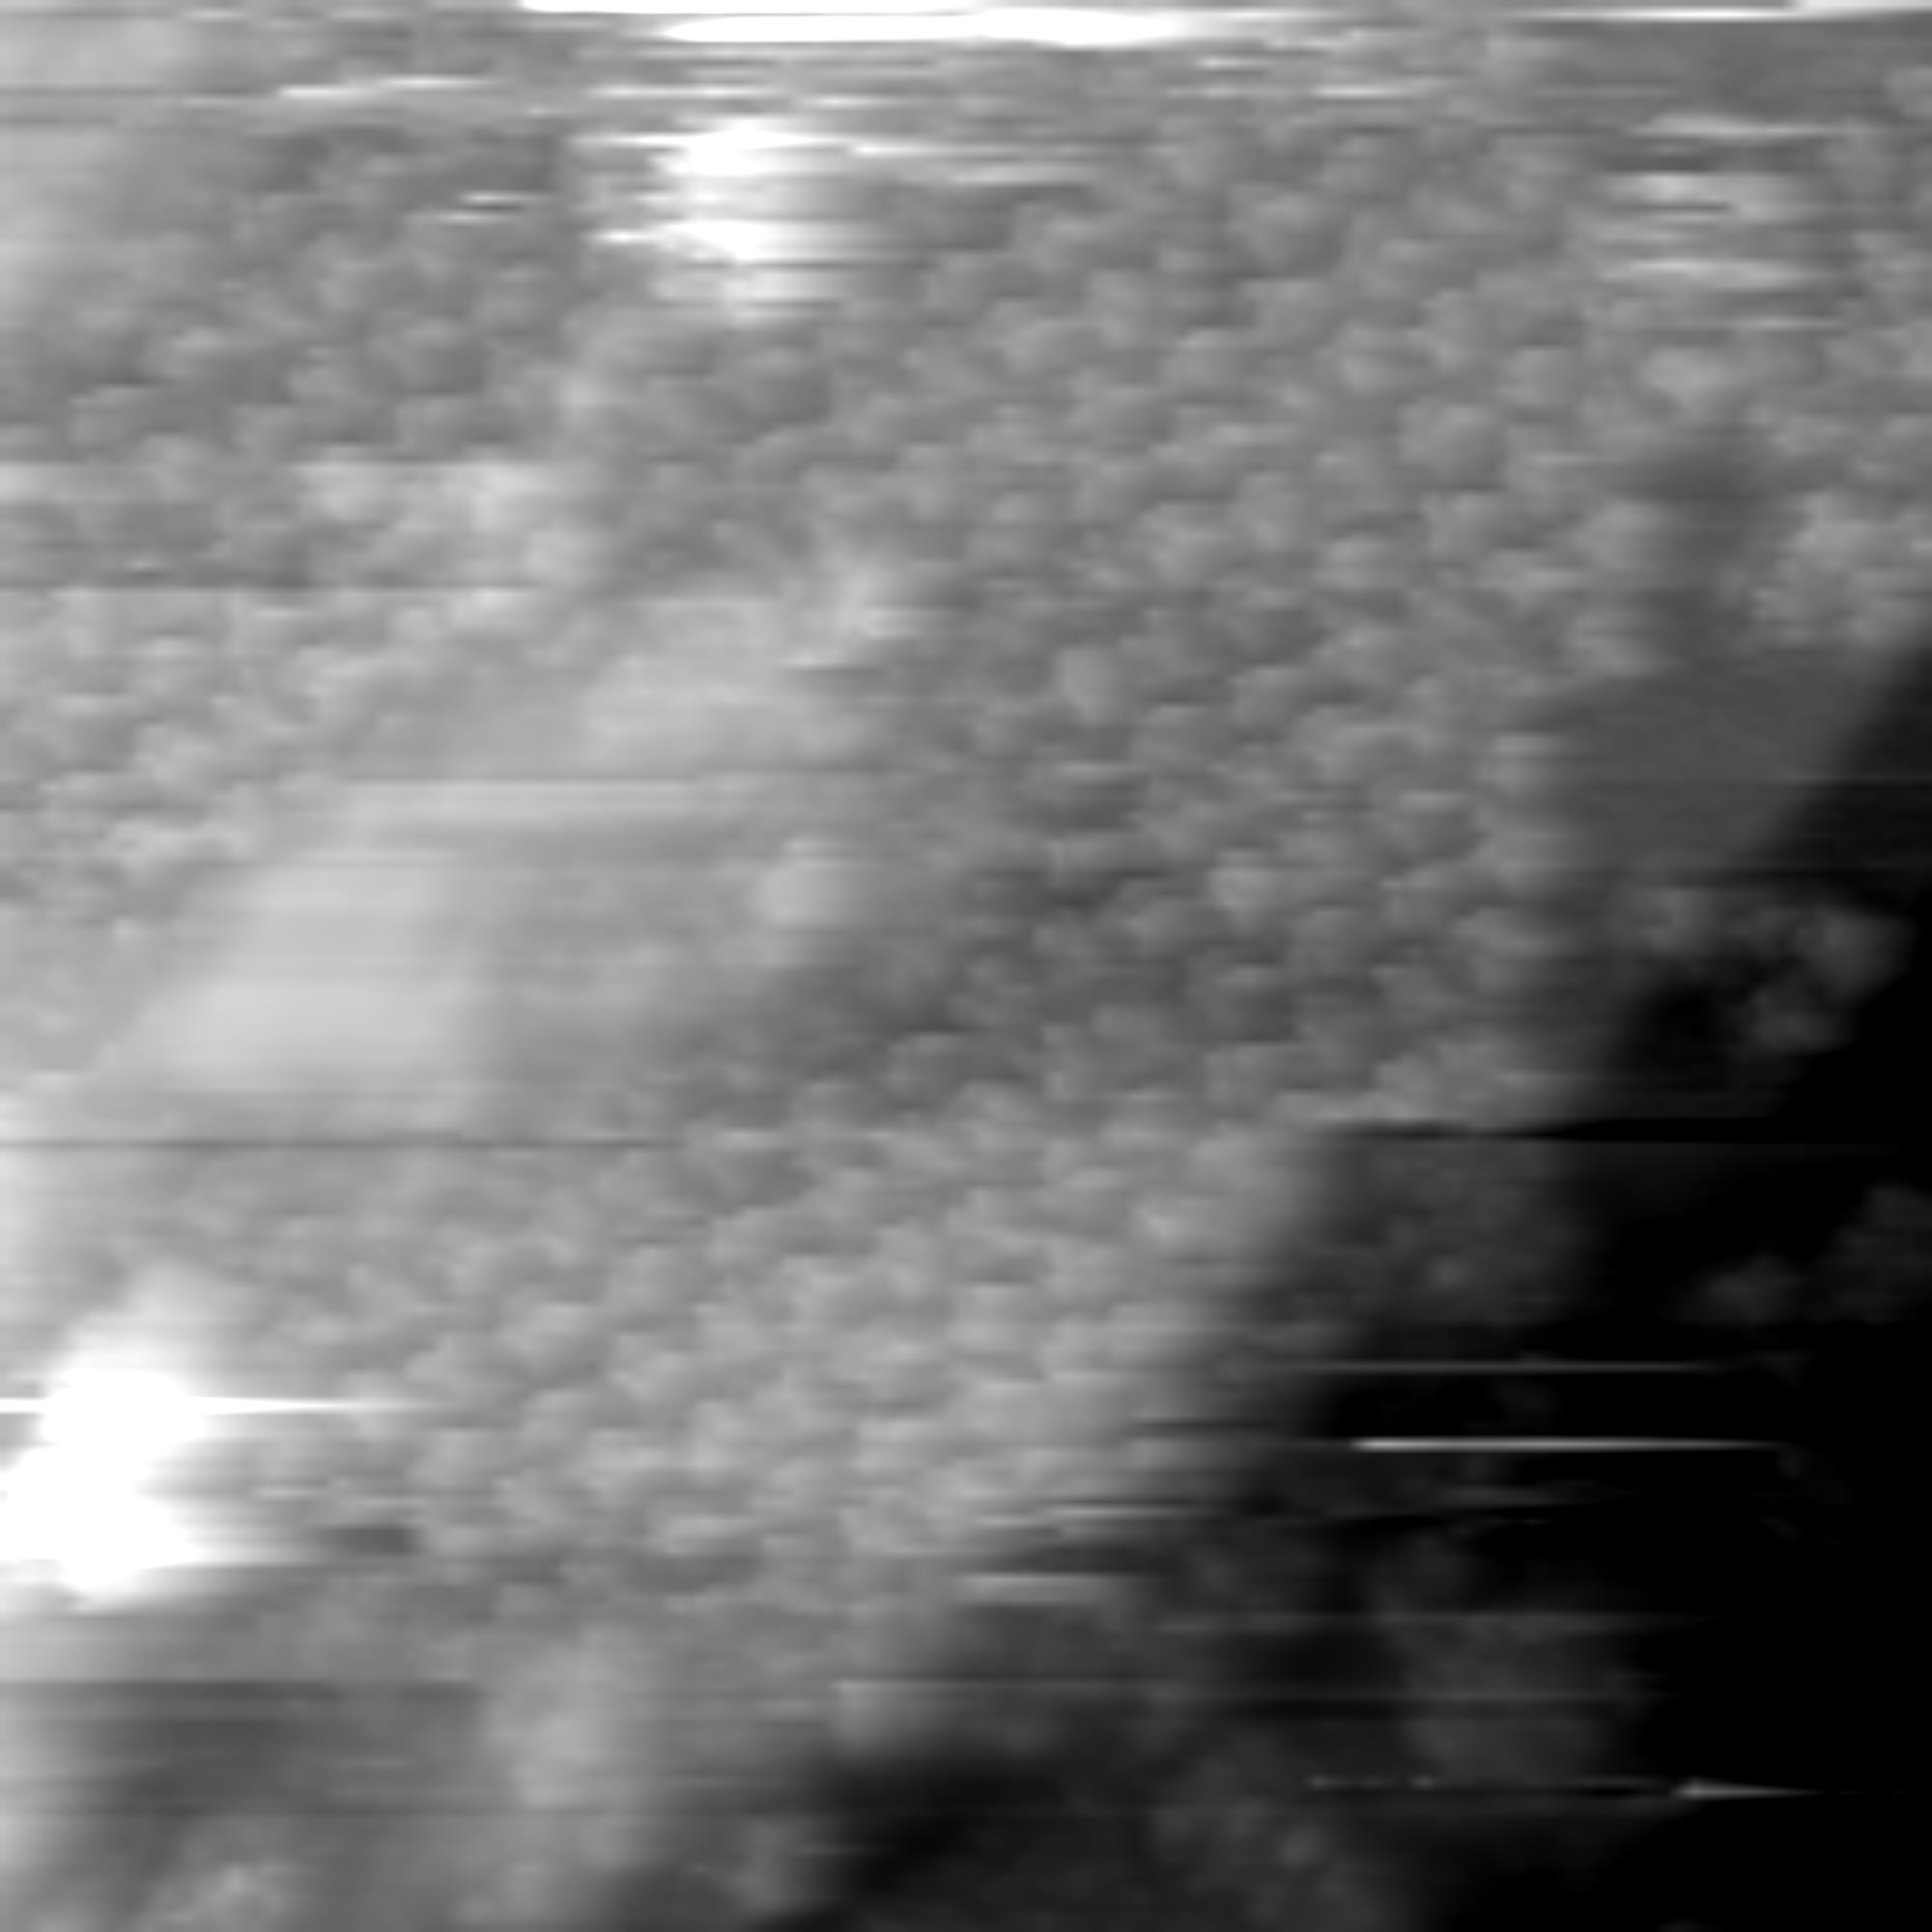
\includegraphics[width=0.5\textwidth]{./images/F151007-112800}
 \caption{TBP on Ag(100) showing some ordering}
 \label{fig:hex-TBP-Ag100}
\end{figure}

%-------------- Add graphic to explain!-------------- 
